\begin{Pro}
Del ejercicio anterior, utiliza las regex de las expresiones booleanas para definir el AF, conviértelo en AFD y redúcelo. Pruébalo con las siguientes expresiones para obtener los tokens:

\begin{enumerate}
    \item[(a)] $p \land q$
    \item[(b)] $\textbf{True} \land \lnot(p \lor q)$
    \item[(c)] $\lnot(x \land y) \lor (p \land q)$
\end{enumerate}

\end{Pro}


Para convertirlo en AF usando Thompson creamos un estado inicial y un estado final, y vamos añadiendo los estados y transiciones según las regex que definimos en el ejercicio anterior. Con lo que obtenemos:

\begin{figure}[H]
    \centering
    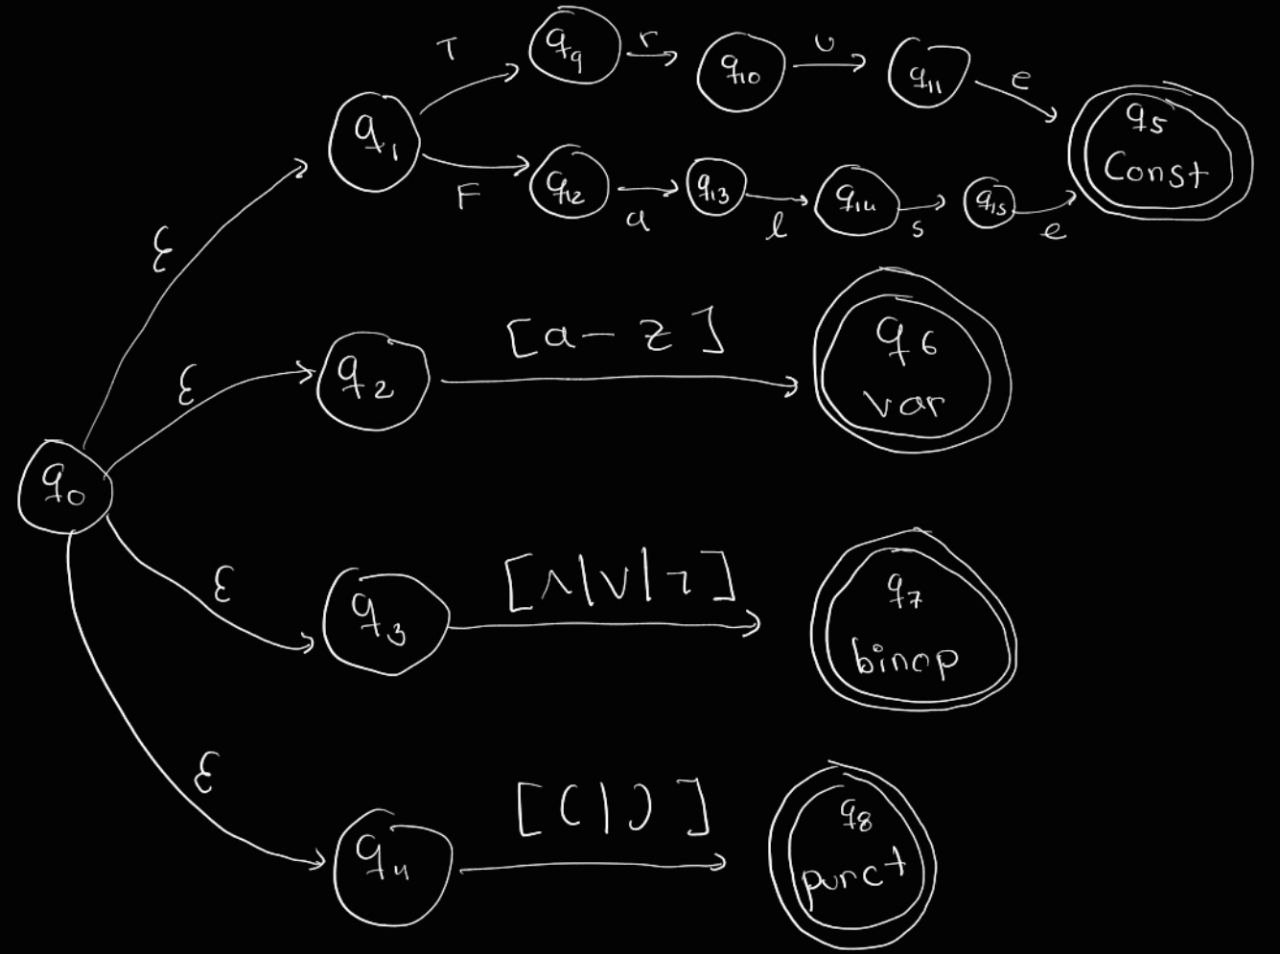
\includegraphics[width=0.8\textwidth]{images/ejercicio10-1.jpg}
    \caption{AF para lexer expresiones booleanas}
    \label{fig:my_label}
\end{figure}